\subsection{Visual Programming Scalability}%
\label{sec:related.ad.vpl-scalability}

Both Dynamo and Grasshopper's visual approach suffer from the disproportionate
scalability between the code and the respective model's
complexity~\cite{Leitao:2013:PESLGD}.  Sophisticated modeling workflows tend to
become difficult to properly represent, and harder for a human to efficiently
interpret when compared to a textual approach.

As an example, consider the Irina Viner-Usmanova \ac{RGC}, a project developed
by TPO Pride\footnote{\url{http://prideproject.pro} (July 2, 2021)} over the
span of three years, from 2016 to 2019.  The \ac{RGC}, built in Moscow's
Luzhniki Stadium, is an arena that houses training sessions and competitions
while also comprising several other premises.
\Cref{fig:related.ad.vpl-scalability.rgc} depicts an outside view of the
\ac{RGC} and its prominent overarching roof covering.  The roof covering was
designed using a combination of Rhino3D and Grasshopper.  Grasshopper was used
from a conceptual stage all the way through to production of construction
drawings.

\begin{figure}[htbp]
  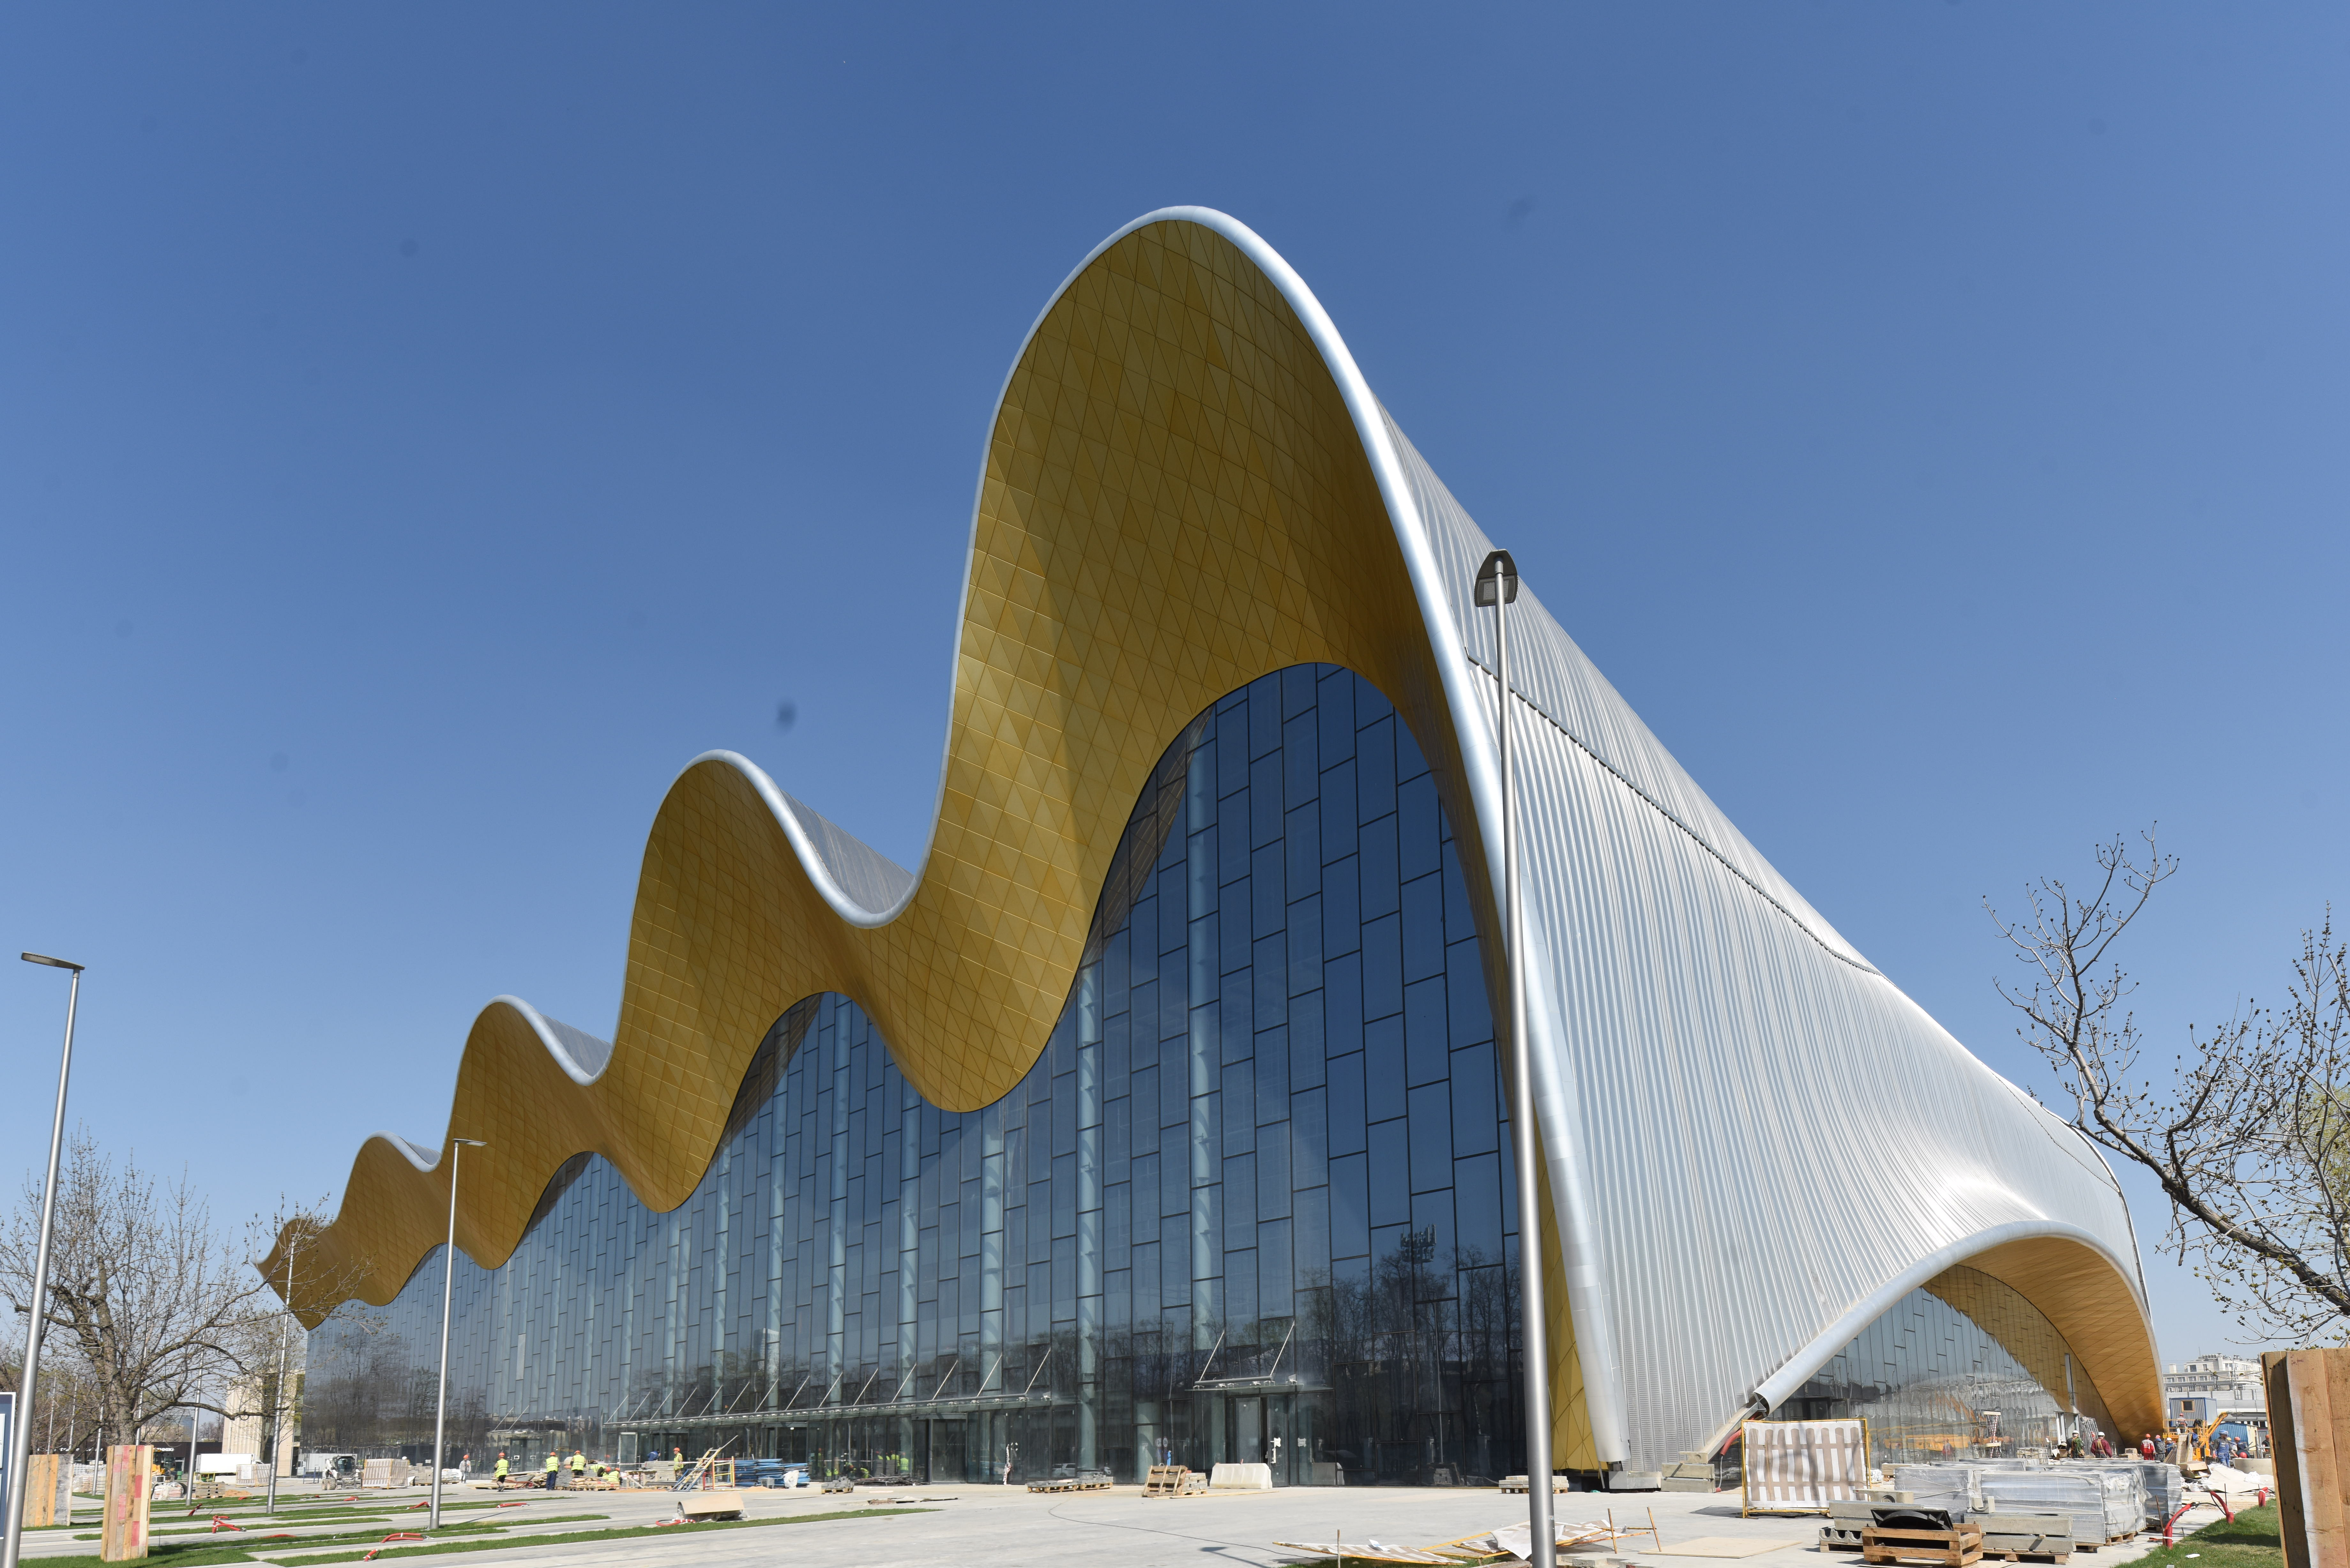
\includegraphics[width=\textwidth]{fig/rgc}\\
  {\scriptsize
  Source: \url{https://www.grasshopper3d.com/photo/rhythmic-gymnastics-center-moscow-russia-5}
  (Jul 2021)
  }
  \caption[\acl{RGC} in the Luzhniki Complex]{
    Irina Viner-Usmanova \ac{RGC} in the Luzhniki Complex, Moscow, Russia.  The
    roof covering was designed using Rhino/Grasshopper.}
  \label{fig:related.ad.vpl-scalability.rgc}
\end{figure}

Developing a roof covering with such a contour lends itself well to \ac{AD}
since it resembles a sine wave whose amplitude is progressively dampened along
the length of the building.  Such a shape can be easily described through a
relatively simple mathematical function to obtain the general wave's shape.
With parametrization in mind, one could then easily fluctuate input variables in
order to achieve different variations of the roof covering's shape, e.g.,
varying the underlying wave's frequency, amplitude, or dampening rate.

Such complex \ac{AD} projects hide equally, if not more, complex corresponding
programs.  The final Grasshopper definition of the \ac{RGC} roof's covering can
be seen in \cref{fig:related.ad.vpl-scalability.rgc-gh}.  This further
reinforces the statement that complex workflows become exponentially difficult
to comprehend due to the added dimensionality of the constructs used in
\acp{VPL}.  This disadvantage, however, is mitigated with their respective
\ac{TPL} alternatives which, despite project complexity, scale relatively better
than \acp{VPL} as the former rely on text, which is one-dimensional, while the
latter rely on boxes and interconnecting wires, which are two-dimensional.

\begin{figure}[htbp]
  \includegraphics[width=\linewidth]{fig/rgc-gh}\\
  {\scriptsize
  Source: \url{https://www.grasshopper3d.com/photo/final-definition} (Jul 2021)
  }
  \caption[Grasshopper definition of the \acl{RGC} roof covering]{
    Final Grasshopper definition of the Irina Viner-Usmanova \ac{RGC} roof
    covering.
  }
  \label{fig:related.ad.vpl-scalability.rgc-gh}
\end{figure}
